\section{Static analysis}

The concept behind static analysis involves examining the source code using analyzers, each tailored to assess a predetermined set of hard-coded (non-custom) properties in a fully automated manner.
The output is deemed safe when no issues are detected and unsafe otherwise.
The properties scrutinized typically revolve around general safety considerations, aiming to prevent conditions that could lead to errors. 
Commonly desired properties include:
\begin{itemize}
    \item Absence of integer variable overflow.
    \item No type errors.
    \item Prevention of null-pointer dereferencing.
    \item Avoidance of out-of-bound array accesses.
    \item Elimination of race conditions.
    \item Prohibition of useless assignments.
    \item Prevention of the use of undefined variables.
\end{itemize}
\begin{definition}[\textit{Program behavior}]
    Program behavior encompasses the entire set of possible executions represented as sequences of states.
\end{definition}
While static analysis is adept at identifying erroneous states, it tends to be pessimistic as the program behavior might not reach any of these states.

\paragraph*{Precision and efficiency}
Static analysis relies on over-approximations to ensure soundness. 
Achieving perfect precision is often unattainable due to undecidability.
The trade-off between precision and efficiency is a critical consideration, as high precision may be computationally expensive, while low precision leads to more false positives that necessitate manual verification.
Designing a static analysis technique involves striking a practical balance between precision and efficiency.

\subsection{Data-flow analysis}
\paragraph*{Control-flow graph}
The control-flow graph (CFG) is a directed graph that depicts potential execution paths in a program.
Each node within the graph represents a program statement, and consecutive statements are connected by edges.
Declarations are disregarded as they do not impact the program state.

\paragraph*{Data-flow analysis}
Data-flow analysis operates on the control-flow graph (CFG) of a program to extract information about the data flow, specifically checking which values are read (used) and written (defined).
The analysis of these properties involves examining the output.
\begin{definition}[\textit{Live variable}]
    In the context of a CFG, a variable $v$ is considered live at the exit of a block $b$ if there exists a path on the CFG from block $b$ to a use of $v$ that does not redefine $v$.
\end{definition}
Live variable analysis determines, for each block, the variables that may be live at the block's exit.
It's crucial to note that the phrase may be live constitutes an over-approximation. 
Thus, $\text{LV}(k)$ represents a superset of the live variables at $k$:
\begin{itemize}
    \item If $x\notin\text{LV}(k)$, then $x$ is definitely not live at $k$. 
    \item If $x\in\text{LV}(k)$, then $x$ may not be live at $k$.
\end{itemize}
The live variable analysis is translated into an equation system, and solving this system identifies the live variables.
Standard algorithms such as fixed-point or worklist can be employed to automatically compute the solution.
Data-flow analysis is effective in eliminating dead assignments; if a variable is not live after being defined by an assignment, that assignment is redundant and can be safely removed without altering the program's behavior.

\paragraph*{Reaching definition analysis}
Reaching definition analysis determines, for each block, the definitions that may reach the block.
\begin{definition}[\textit{Definition}]
    A definition $(v,k)$ represents an assignment to variable $v$ occurring at block $k$. 
\end{definition}
\begin{definition}[\textit{Block reachability}]
    A definition $(v,k)$ reaches block $r$  if there exists a path from $k$ to $r$ that does not redefine $v$.
\end{definition}
For this type of analysis, the following equations can be defined for each block $k$: 
\[\text{RD}_{\text{IN}}(k)= \bigcup_{h \rightarrow k}\text{RD}_{\text{OUT}}(h)\]
\[\text{RD}_{\text{OUT}}(k)= \left(\text{RD}_{\text{IN}}(k) - \text{kill}_{\text{RD}}(k) \right) \cup \text{Gen}_{\text{RD}}(k)\]
Reaching definition analysis provides information about which statements define values and which use them, making it valuable for program optimizations or error avoidance.
\begin{definition}[\textit{Use-definition chain}]
    A use-definition chain, denoted as UD, links a use to all definitions that may reach it:
    \[\text{UD}(v,k)=\{q|{"q:v:=E"} \textnormal{ and def\_clear}(v,q,k)\}\cup\{?|\text{def\_clear}(v,?,k)\}\]
\end{definition}
Here, "q:v:=E" is an assignment for $v$ at line $q$. 
$\text{def\_clear}(v,q,k)$ holds if and only if there is a definition-clear path from $q$ to $k$ (i.e., no block between $q$ and $k$ redefines $v$).
\begin{definition}[\textit{Use-definition path}]
    A use-definition path is a path from $q$ to $k$ such that $k$ uses some $v$ and $q \in \text{UD}(v,k)$.
\end{definition}
The set $\text{UD}(v, k)$ can be computed from reaching definitions analysis as follows: 
\[\begin{cases}
    \{q|(v,q)\in \text{RD}_{\text{IN}}(k)\} \textnormal{ if }v \textnormal{ uses } d \textnormal{ in block } k \\
    \{\:\} \textnormal{ otherwise}
\end{cases}\]
\begin{definition}[\textit{Definition-use chain}]
    A definition-use chain, denoted as DU, links a definition to all use such that the definition may reach them:
    \[\text{DU}(v,k)=\{q|q \textnormal{ uses } v \textnormal{ and } (v,k) \textnormal{ reaches } q\}\]
\end{definition}
\begin{definition}[\textit{Definition-use path}]
    A definition-use path is a path from $k$ to $q$ such that $k$ defines some $v$ and $q \in \text{DU}(v,k)$.
\end{definition}
The set $\text{DU}(v, k)$ can be computed as the inverse of use definition: 
\[ \text{DU}(v,k)=\{q|k \in \text{UD}(v,q)\}\]
\begin{definition}[\textit{Definition-use pair}]
    Given $\text{DU}(v,k)$, if some $q \in \text{DU}(v, k)$, we say that $\left\langle k,q \right\rangle $ is a definition-use pair for $v$.
\end{definition}
\begin{example}
    Let's examine the given code snippet:
    \begin{lstlisting}[style=Java]
int foo() {
    x = input();
    while (x > 0) {
        y = 2 * x;
        if (x > 10)
            y = x - 1;
        else
            x = x + 2;
            x = x - 1;
    }
    x = x - 1;
    return x;
}  
    \end{lstlisting}
    We initiate the analysis by constructing the control flow graph (CFG) of the program:
    \begin{figure}[H]
        \centering
        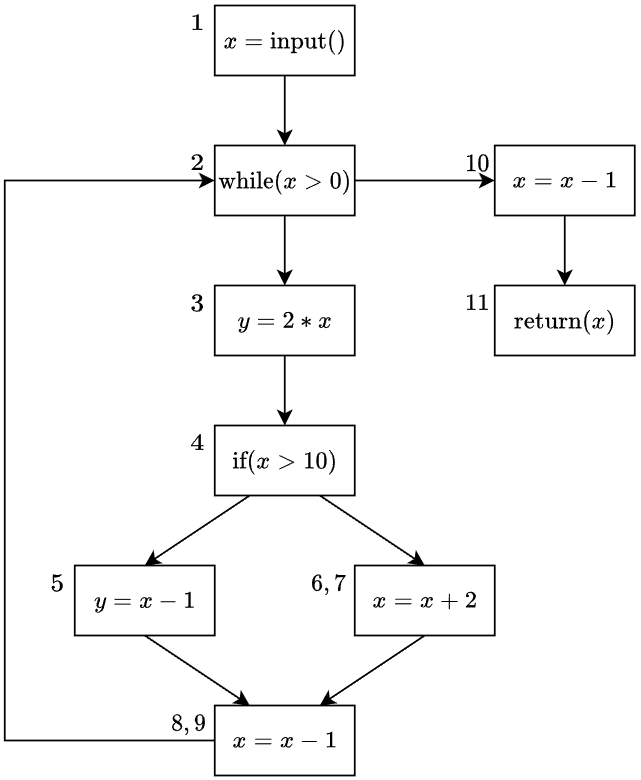
\includegraphics[width=0.5\linewidth]{images/cfg.png}
    \end{figure}
    Utilizing the CFG, we conduct live variable analysis, resulting in:
    \begin{itemize}
        \item $\text{LV}(1)=\{x\}$.
        \item $\text{LV}(2)=\{x\}$.
        \item $\text{LV}(3)=\{x\}$, there is a problem since $y$ is defined here and not live. 
        \item $\text{LV}(4)=\{x\}$.
        \item $\text{LV}(5)=\{x\}$, there is a problem since $y$ is defined here and not live. 
        \item $\text{LV}(6,7)=\text{LV}(8,9)=\text{LV}(10)=\{x\}$.
        \item $\text{LV}(11)=\{\:\}$.
    \end{itemize}
    Using the CFG, we also establish definition-use pairs:
    \begin{itemize}
        \item $\text{RD}_{\text{IN}}(1) = \{ (x,?), (y,?) \}$.
        \item $\text{RD}_{\text{IN}}(2) = \text{RD}_{\text{OUT}}(1) \cup \text{RD}_{\text{OUT}} (8,9) = \{ (x,1), (y,?), (x,8), (y, 5), (y, 3) \}$.
        \item $\text{RD}_{\text{IN}}(3) = \text{RD}_{\text{OUT}}(2) = \{ (x,1), (y,?) , (x, 8), (y, 5), (y, 3)\}$.
        \item $\text{RD}_{\text{IN}}(4) = \text{RD}_{\text{OUT}}(3) = \{ (x,1), (x, 8), (y, 3)\}$.
        \item $\text{RD}_{\text{IN}}(5) = \text{RD}_{\text{OUT}}(4) = \{ (x,1), (x, 8), (y, 3)\}$.
        \item $\text{RD}_{\text{IN}}(6,7) = \text{RD}_{\text{OUT}}(4) =\{ (x,1), (x, 8), (y, 3)\}$.
        \item $\text{RD}_{\text{IN}}(8,9) = \text{RD}_{\text{OUT}}(5) \cup \text{RD}_{\text{OUT}}(6,7) = \{ (x,1), (y, 5), (x,7), (x, 8), (y, 3) \}$.
        \item $\text{RD}_{\text{IN}}(10) = \text{RD}_{\text{OUT}}(2) = \{ (x,1), (y,?) , (x, 8), (y, 5), (y,3)\}$.
        \item $\text{RD}_{\text{IN}}(11) = \text{RD}_{\text{OUT}}(10) = \{ (x,10), (y,?) , (y, 5), (y, 3)\}$.
    \end{itemize}
    Based on these definitions, we establish the used definition chains and the definition-use pairs. 
    We observe that $x$ is defined in 1, 7, 8, 10 and used in 2, 3, 4, 5, 7, 8, 10, 11, and $y$ is defined in 3, 5 but not used. 
    The use definition chains are defined as follows:
    \begin{enumerate} 
        \item $\text{UD}(x, 2) = UD(x, 3) = UD(x, 4) = UD(x, 5) = UD(x, 7) = UD(x, 10) = \{1, 8\}$
        \item $\text{UD}(x, 8) = \{1, 7, 8\}$
        \item $\text{UD}(x, 11) = \{10\}$
    \end{enumerate} 
    Consequently, the definition-use pairs for $x$ are:
    \begin{enumerate}
        \item $\left\langle 1,2 \right\rangle$, $\left\langle 1,3 \right\rangle$, $\left\langle 1,4 \right\rangle$, $\left\langle 1,5 \right\rangle$, $\left\langle 1,7 \right\rangle$, $\left\langle 1,8 \right\rangle$, and $\left\langle 1,10 \right\rangle$.
        \item $\left\langle 7,8 \right\rangle$.
        \item $\left\langle 8,2 \right\rangle$, $\left\langle 8,3 \right\rangle$, $\left\langle 8,4 \right\rangle$, $\left\langle 8,5 \right\rangle$, $\left\langle 8,7 \right\rangle$, $\left\langle 8,8 \right\rangle$, and $\left\langle 8,10 \right\rangle$.
        \item $\left\langle 10,11 \right\rangle$.
    \end{enumerate}
\end{example}

\subsection{Symbolic execution}
Symbolic execution is an approach that scrutinizes source code to assess specific properties. 
The key properties examined include:
\begin{itemize}
    \item \textit{Reachability}: this involves determining whether a particular location $l$ in the code $S$ is reachable in any execution. 
        The method aims to verify that $l$ is unreachable in some executions or identifies the conditions under which $l$ becomes reachable.
    \item \textit{Path feasibility}: this property involves checking whether a specific path $p$ in the code $S$ is entirely reachable. 
        The objective is to confirm that the execution of $p$ is not possible, or alternatively, identify the conditions under which $p$ can be executed.
\end{itemize} 
Symbolic execution can be employed for automatic test case generation. 
However, it may fall short of identifying all possible paths.
The process involves executing programs with symbolic values, and symbolic states keep track of the symbolic values of variables.
The potential outcomes of symbolic execution are:
\begin{itemize}
    \item SAT exit ($\pi$ is satisfiable): indicates that there exists a satisfying assignment to variables in $\pi$ and such an assignment represents an input that satisfies the specified property in a concrete execution.
    \item UNSAT exit ($\pi$ is not satisfiable): denotes that the given property cannot be satisfied by any concrete execution.
\end{itemize}
Execution paths can be organized into an execution tree, with final states marked as SAT or UNSAT.
\begin{example}
    Consider the provided code snippet:
    \begin{lstlisting}[style=Java]
int foo(int x, int y) {
    int z := x
    if (z < y)
        z := z*2
    if (x < y && z >= y)
        print(z) 
}
    \end{lstlisting}
    In line zero, two variables, $x$ and $y$, are defined. 
    Consequently, we initialize a table with these variables having symbolic values $X$ and $Y$, respectively. 
    Line zero is added to the path as it is always executed.
    \begin{table}[H]
        \centering
        \begin{tabular}{l|lll}
        \textbf{Symbolic state}  & $x$ & $y$ &  \multirow{2}{*}{$\left\langle 0\right\rangle $} \\ \cline{1-3}
        \textbf{Symbolic values} & $X$ & $Y$ &                      
        \end{tabular}
    \end{table}
    In line one, a new variable $z$ is defined with the same value as $x$.
    We add a state $z$ with a value of $X$ and include line one in the path as it is always reachable.
    \begin{table}[H]
        \centering
        \begin{tabular}{l|llll}
        \textbf{Symbolic state}  & $x$ & $y$ & $z$ & \multirow{2}{*}{$\left\langle 0,1 \right\rangle $} \\ \cline{1-4}
        \textbf{Symbolic values} & $X$ & $Y$ & $X$ &                     
        \end{tabular}
    \end{table}
    In line two, a conditional expression is encountered, which is always checked. 
    Thus, we add $2$ to the path and introduce a state $\pi$ to represent the condition. 
    The table becomes duplicated based on the condition:
    \begin{table}[H]
        \centering
        \begin{tabular}{l|ccccc}
        \textbf{Symbolic state}  & $x$ & $y$ & $z$ & $\pi$ & \multirow{2}{*}{$\left\langle 0,1,2 \right\rangle $} \\ \cline{1-5}
        \textbf{Symbolic values} & $X$ & $Y$ & $X$ & $X<Y$ &                    
        \end{tabular}
    \end{table}
    \begin{table}[H]
        \centering
        \begin{tabular}{l|ccccc}
        \textbf{Symbolic state}  & $x$ & $y$ & $z$ & $\pi$ & \multirow{2}{*}{$\left\langle 0,1,2 \right\rangle $} \\ \cline{1-5}
        \textbf{Symbolic values} & $X$ & $Y$ & $X$ & $X\geq Y$ &                    
        \end{tabular}
    \end{table}
    Since symbolic execution prioritizes feasible paths, we select the first table. 
    In line three, the value of $z$ is redefined, and the path now reaches line three:
    \begin{table}[H]
        \centering
        \begin{tabular}{l|ccccc}
        \textbf{Symbolic state}  & $x$ & $y$ & $z$ & $\pi$ & \multirow{2}{*}{$\left\langle 0,1,2,3 \right\rangle $} \\ \cline{1-5}
        \textbf{Symbolic values} & $X$ & $Y$ & $2X$ & $X<Y$ &                    
        \end{tabular}
    \end{table}
    Another condition on the $\pi$ column is added, resulting in two tables:
    \begin{table}[H]
        \centering
        \begin{tabular}{l|ccccc}
        \textbf{Symbolic state}  & $x$ & $y$ & $z$ & $\pi$ & \multirow{2}{*}{$\left\langle 0,1,2,3,4 \right\rangle $} \\ \cline{1-5}
        \textbf{Symbolic values} & $X$ & $Y$ & $2X$ & \makecell{$X<Y$ \\ $X < Y \land 2X \geq Y$} &                    
        \end{tabular}
    \end{table}
    \begin{table}[H]
        \centering
        \begin{tabular}{l|ccccc}
        \textbf{Symbolic state}  & $x$ & $y$ & $z$ & $\pi$ & \multirow{2}{*}{$\left\langle 0,1,2,3,4 \right\rangle $} \\ \cline{1-5}
        \textbf{Symbolic values} & $X$ & $Y$ & $2X$ & \makecell{$X<Y$ \\ $X < Y \land 2X \geq Y$} &                    
        \end{tabular}
    \end{table}
    We again select the path that satisfies the condition, resulting in:
    \begin{table}[H]
        \centering
        \begin{tabular}{l|ccccc}
        \textbf{Symbolic state}  & $x$ & $y$ & $z$  & $\pi$                                         & \multirow{2}{*}{$\left\langle 0,1,2,3,4,5 \right\rangle $} \\ \cline{1-5}
        \textbf{Symbolic values} & $X$ & $Y$ & $2X$ & \makecell{$X<Y$ \\ $X < Y \land 2X \geq Y$}   &                    
        \end{tabular}
    \end{table}
    We observe that location five is reachable by assigning the appropriate values to the variables ($X=2$, $Y=3$).
    Additionally, the path $\left\langle 0,1,2,4,5 \right\rangle$ is not feasible since there is no satisfying assignment.
\end{example}
Execution paths can be organized into an execution tree, with conclusive states marked as SAT (satisfiable) or UNSAT (unsatisfiable). 
While symbolic execution offers a promising approach for verifying program correctness, certain challenges exist:
\begin{itemize}
    \item \textit{Complex path conditions}: path conditions generated during symbolic execution may become overly intricate for constraint solvers. 
        While solvers excel at handling linear constraints, their proficiency diminishes when faced with non-linear arithmetic, bit-wise operations, or string manipulation.
    \item \textit{Handling large path spaces}: symbolic execution encounters difficulties when the number of paths to explore becomes substantial. 
        Unbounded loops, in particular, introduce infinite sets of paths. 
        Even if the path set is finite, examining all loop iterations can be impractical. 
        A common strategy is to approximate the analysis by considering 0, 1, and 2 iterations as a practical rule of thumb.
    \item \textit{External code and unavailability of sources}: the presence of external code, especially when the source code is not accessible, introduces uncertainty in the solver's understanding of behavior. 
        This can pose challenges as the solver may lack crucial information to reason about the program accurately.
\end{itemize}